% =====================================================================
% ARS-Stack — research paper draft, single-column format
% Build: see paper/build.sh (tectonic main.tex), or upload this folder to Overleaf.
% =====================================================================
\documentclass[10pt]{article}

\usepackage[a4paper, margin=1in]{geometry}
\usepackage{iftex}
\ifPDFTeX
  \usepackage[T1]{fontenc}
  \usepackage{lmodern}
\fi
\usepackage{microtype}
\usepackage{amsmath, amssymb}
\usepackage{graphicx}
\usepackage{booktabs, tabularx, multirow}
\usepackage{xcolor}
\usepackage{tikz}
\usetikzlibrary{positioning, fit, arrows.meta, calc}
\usepackage{algorithm}
\usepackage{algpseudocode}
\usepackage[numbers, sort&compress]{natbib}
\usepackage[font=small, labelfont=bf]{caption}
\usepackage[hidelinks]{hyperref}
\usepackage{authblk}

\newcommand{\ars}{ARS-Stack}
% Run-in paragraph heading (IEEEtran appends its own colon, article does not).
\newcommand{\para}[1]{\paragraph{#1.}}
% Content shown only in the longer single-column version.
\newif\iffullversion
\fullversiontrue
% Wide floats: ordinary floats in single-column layout (figure* / table* in the IEEE version).
\newenvironment{widefigure}{\begin{figure}}{\end{figure}}
\newenvironment{widetable}{\begin{table}}{\end{table}}
\newcommand{\usagefigwidth}{0.66\linewidth}
\newcommand{\protocolfigwidth}{0.62\linewidth}
% Float placement: allow floats "here" and fill pages densely.
\makeatletter
\renewcommand{\fps@figure}{!htbp}
\renewcommand{\fps@table}{!htbp}
\renewcommand{\fps@algorithm}{!htbp}
\makeatother
\renewcommand{\topfraction}{0.9}
\renewcommand{\bottomfraction}{0.8}
\renewcommand{\textfraction}{0.07}
\renewcommand{\floatpagefraction}{0.85}
\setcounter{topnumber}{3}
\setcounter{bottomnumber}{2}
\setcounter{totalnumber}{4}

\title{\textbf{Does Adaptive Resampler Selection Help Modern Tree Ensembles?\\
ARS-Stack and a Controlled Study on 28 Imbalanced Datasets}}
\author[1]{[Author Name]}
\author[1]{[Co-author Name]}
\affil[1]{[Department, Institution, City, Country]\\ \texttt{[email@institution.edu]}}
\date{Draft --- \today}

\begin{document}
\maketitle

\begin{abstract}
Class imbalance is usually handled by resampling the training data and then fitting an ensemble. Most hybrid
pipelines apply one resampler to the whole minority class and combine their learners with fixed weights. We
propose \ars{} (Adaptive Resampler-Selection Stacking), which clusters the minority class, scores each cluster
for class overlap and local density, selects a resampler \emph{per cluster}, and combines Random Forest, XGBoost and
LightGBM with confidence weights. We evaluate it under a leakage-free, budget-matched protocol on 28 datasets
(credit-card fraud, mammography, 10-class yeast and 25 benchmarks) against eight baselines and ablations: 3,780
cross-validation folds, analysed with frequentist and Bayesian tests. \ars{} is significantly and practically better
than global SMOTE-ENN (Bayesian probability $\geq 0.96$ on F1, AUC-PR and MCC). It is, however, \emph{practically
equivalent} to plain SMOTE, SMOTE-Tomek and its own ablations, and it cannot be separated from training without
resampling. Diagnostics explain why: the confidence weights are almost uniform, Tomek cleaning removes nothing after
1:1 SMOTE, and the selector rarely varies its choice within a dataset. A pilot of validated selection closes the gap
to the baselines but does not exceed them. Resampling helps mainly when the minority class is very small (mean
AUC-PR gain $+0.012$ below 75 minority samples, $-0.009$ above). We release the reproducible pipeline and discuss
five evaluation pitfalls that make new resamplers look better than they are.

\end{abstract}

\noindent\textbf{Keywords:} class imbalance, resampling, SMOTE, ensemble learning, stacking, statistical comparison
of classifiers, Bayesian analysis, MLOps.

\section{Introduction}\label{sec:intro}

In fraud detection, medical screening, intrusion detection and churn prediction, the class of interest is usually
the rarest. A classifier that minimises overall error can then reach high accuracy while missing most minority cases,
which keeps class imbalance a central problem in applied machine learning~\cite{he2009learning,krawczyk2016learning,
branco2016survey,fernandez2018book}. The standard remedies are \emph{data-level} resampling, which generates synthetic
minority samples or removes majority ones~\cite{chawla2002smote,he2008adasyn,batista2004study}, and ensembles that
reduce the variance and bias of minority predictions~\cite{galar2012review,chawla2003smoteboost,liu2009exploratory}.
Hybrid pipelines that resample the data and then fit an ensemble dominate recent applied work, particularly on
credit-card fraud~\cite{plan_p7_comparative,plan_p9_fraud,plan_p10_stacking}.

Our literature review (Section~\ref{sec:related}) found three recurring gaps. First, one resampler is chosen by hand
and applied \emph{uniformly} to the whole minority class, although the best resampler depends on the
dataset~\cite{plan_p8_hybrid,kovacs2019empirical} and plausibly on the region: small disjuncts~\cite{jo2004class},
borderline points~\cite{han2005borderline} and overlap zones~\cite{plan_p2_dcshs} each call for different treatment.
Second, ensemble combiners are static and trust every learner equally~\cite{plan_p5_survey}. Third, multiclass
imbalance is under-studied~\cite{plan_p3_multiclass,plan_p6_smoteif}.

We designed \ars{} to address all three. It clusters each minority class, scores the clusters for overlap and
density, picks a resampler per cluster, and combines Random Forest~\cite{breiman2001random},
XGBoost~\cite{chen2016xgboost} and LightGBM~\cite{ke2017lightgbm} with confidence weights. It supports binary and
multiclass problems and ships as a reproducible MLOps system.

Evaluating it fairly proved harder than building it. We found, and removed from our own pipeline, five pitfalls that
each manufacture a spurious improvement: unequal oversampling budgets, confidence weights cancelled by a meta-learner,
rank-forced selection rules, fixed decision thresholds, and duplicate records that straddle train and test splits.
With them removed, we asked whether adaptive resampler selection helps a modern tree ensemble at all. The answer is
largely negative, and we argue that this answer is the more useful result.

\para{Contributions}
\begin{enumerate}
  \item \textbf{Method:} \ars{}, with scale-free cluster scores, a global synthetic-sample budget, confidence-weighted
        averaging with a tuned threshold, and a multiclass extension (Section~\ref{sec:method}).
  \item \textbf{Protocol:} a leakage-free, budget-matched evaluation in which scaling, resampling, weighting and
        thresholds are fitted inside each fold (Section~\ref{sec:setup}).
  \item \textbf{Study:} nine variants on 28 datasets with repeated cross-validation, analysed with Friedman, Nemenyi,
        Holm-corrected Wilcoxon and corrected resampled $t$-tests, and with Bayesian tests using a region of
        practical equivalence~\cite{benavoli2017time} (Section~\ref{sec:results}).
  \item \textbf{Diagnosis:} why each component does or does not help, a validated-selection pilot, and a meta-analysis
        of when resampling helps (Section~\ref{sec:analysis}).
  \item \textbf{Artifact:} an open pipeline (DVC, MLflow~\cite{zaharia2018accelerating}, Prefect, Docker, CI,
        FastAPI) that records code version, packages and hardware with every result.
\end{enumerate}

In short, \ars{} beats aggressive cleaning (SMOTE-ENN) but is practically equivalent to plain SMOTE and to its
ablations, and it cannot be separated from no resampling. This agrees with growing evidence that strong learners
gain little from oversampling~\cite{elor2022smote,vandengoorbergh2022harm,vanhulse2007experimental}.

\section{Related Work and Research Gaps}\label{sec:related}

\para{Resampling}
SMOTE~\cite{chawla2002smote} interpolates between a minority sample and one of its $k$ nearest minority neighbours and
remains the default oversampler~\cite{fernandez2018smote}. Its descendants mainly change \emph{where} samples are
placed. Borderline-SMOTE~\cite{han2005borderline} and ADASYN~\cite{he2008adasyn} focus on hard points; Safe-Level
SMOTE~\cite{bunkhumpornpat2009safe} and MWMOTE~\cite{barua2014mwmote} avoid noisy regions; $k$-means
SMOTE~\cite{douzas2018kmeans} generates only inside safe clusters. Cleaning methods remove ambiguous points:
Tomek links~\cite{tomek1976two} delete cross-class nearest-neighbour pairs, and ENN~\cite{wilson1972asymptotic} removes
points misclassified by their neighbours. Both were combined with SMOTE by Batista \emph{et al.}~\cite{batista2004study}.
In Kov\'{a}cs's comparison of 85 oversamplers on 104 datasets~\cite{kovacs2019empirical}, no method dominates.

\para{Cluster- and region-aware resampling}
The minority class is often a union of sub-concepts, and errors concentrate in small disjuncts~\cite{jo2004class}.
Cluster-based methods~\cite{jo2004class,douzas2018kmeans} and DCSHS~\cite{plan_p2_dcshs}, which uses dual clustering
and stage-wise hybrid sampling in overlap zones, adapt \emph{where} samples are generated. They still apply one fixed
\emph{technique}, however. We found no method that chooses among several resamplers per region.

\para{Ensembles}
Boosting (SMOTEBoost~\cite{chawla2003smoteboost}, RUSBoost~\cite{seiffert2010rusboost}), bagging
(EasyEnsemble~\cite{liu2009exploratory}) and stacking~\cite{wolpert1992stacked} have all been adapted to
imbalance~\cite{galar2012review}. Random Forests and gradient-boosted trees~\cite{breiman2001random,chen2016xgboost,
ke2017lightgbm} are now the usual base learners in hybrid fraud pipelines~\cite{plan_p9_fraud,plan_p10_stacking}.
Instance-adaptive combination is studied as dynamic classifier selection~\cite{cruz2018dynamic}. Resampling pipelines,
however, typically combine their learners with a fixed vote or an unweighted meta-learner~\cite{plan_p5_survey}.

\para{Evaluation}
Under imbalance, precision--recall metrics~\cite{saito2015precision}, the G-mean~\cite{kubat1997addressing} and the
MCC~\cite{chicco2020advantages} replace accuracy. Across datasets, Dem\v{s}ar~\cite{demsar2006statistical} recommends the
Friedman test~\cite{friedman1937use,iman1980approximations} with post-hoc
tests~\cite{nemenyi1963distribution,holm1979simple}. Within a dataset, correlated folds call for the corrected
resampled $t$-test~\cite{nadeau2003inference,bouckaert2004evaluating}. Bayesian tests with a region of practical
equivalence (ROPE)~\cite{benavoli2017time,corani2015bayesian,benavoli2014bayesian} can also support \emph{equivalence}.
Several studies doubt that resampling helps strong learners: gains vanish with boosted trees and tuned
thresholds~\cite{elor2022smote}, imbalance corrections harm calibration~\cite{vandengoorbergh2022harm}, and benefits
depend on the learner~\cite{vanhulse2007experimental}.

\para{Research gaps}
Table~\ref{tab:litgaps} condenses the ten studies of our review into four gaps:
\textbf{G1}, no resampler dominates, yet pipelines fix one globally;
\textbf{G2}, ensemble weights are static;
\textbf{G3}, multiclass imbalance is under-explored;
\textbf{G4}, evidence comes from few datasets and frequentist tests, and rarely controls the amount of resampling or
leakage from resampling before splitting.
\ars{} targets G1--G3; our protocol targets G4.

\begin{widetable}
  \centering
  \caption{Studies from our literature review and the gaps they leave open (mapped to G1--G4).}
  \label{tab:litgaps}
  \scriptsize
  \begin{tabularx}{\linewidth}{@{}l>{\raggedright\arraybackslash}X>{\raggedright\arraybackslash}p{0.2\linewidth}>{\raggedright\arraybackslash}X@{}}
    \toprule
    Ref. & Approach & Data & Limitation / gap \\
    \midrule
    SHREA~\cite{plan_p1_shrea} & Oversample-impute, undersample, one-class classifiers, bagging & Generic benchmarks & No large fraud/medical test; no SMOTE-ENN comparison (G4) \\
    DCSHS~\cite{plan_p2_dcshs} & Dual clustering, stage-wise hybrid sampling in overlap zones & Public imbalanced sets & Region-aware but one sampling scheme (G1) \\
    \cite{plan_p3_multiclass} & Survey: resampling + ensembles, binary vs.\ multiclass & Health, finance, security & 18/24 prior works binary only (G3) \\
    \cite{plan_p4_gradient} & Gradient-based instance-level resampling & Cost-sensitive benchmarks & Tied to boosting internals, hard to reproduce (G4) \\
    \cite{plan_p5_survey} & Spatial-distribution undersampling + voting & Various & Static voting weights (G2) \\
    \cite{plan_p6_smoteif} & SMOTE + Isolation-Forest filtering & Medical multiclass & Medical only; no stacking (G1, G3) \\
    \cite{plan_p7_comparative} & EasyEnsemble, XGBoost, RF, AdaBoost & Fraud, phishing & Benchmarks existing methods only (G1) \\
    \cite{plan_p8_hybrid} & ROS/RUS/hybrid $\times$ bagging/boosting & Water quality & Best resampler dataset-dependent, no selector (G1) \\
    \cite{plan_p9_fraud} & SMOTE + RF/XGBoost/LightGBM/stacking & IEEE-CIS, fraud & Resampler fixed to SMOTE (G1) \\
    \cite{plan_p10_stacking} & SMOTE/SMOTE-Tomek + stacking & Credit-card fraud & One domain, manual resampler (G1, G4) \\
    \bottomrule
  \end{tabularx}
\end{widetable}

\section{The ARS-Stack Method}\label{sec:method}

Figure~\ref{fig:arch} shows the system. The data layer versions and cleans the data. The adaptive-resampling layer,
the methodological core, prepares the training set for the ensemble layer. An MLOps layer makes every run
reproducible. We describe the binary case (minority class $c$) first and then the multiclass extension.

\begin{widefigure}
  \centering
  \resizebox{\linewidth}{!}{% ARS-Stack architecture: data layer -> adaptive resampling -> ensemble -> evaluation/serving,
% with the MLOps layer underneath. Scaled to the available width by the caller.
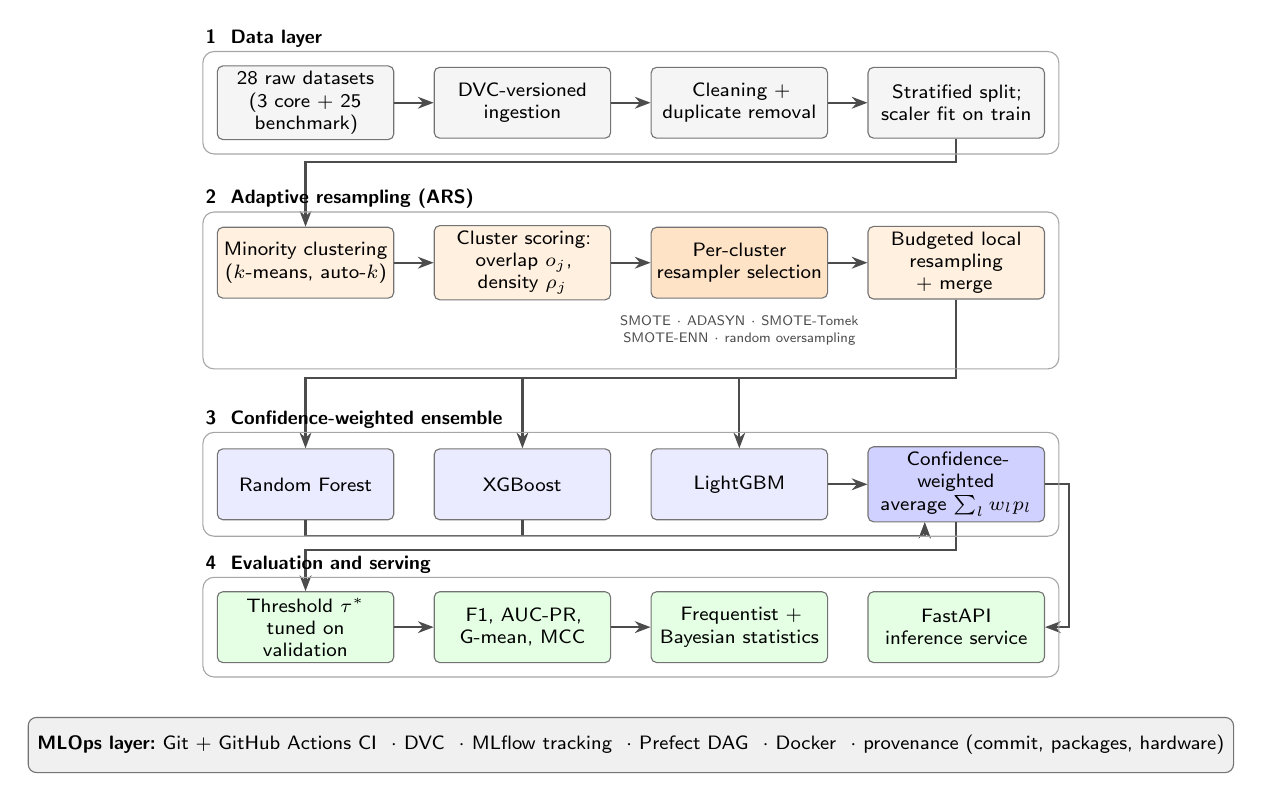
\begin{tikzpicture}[
    font=\sffamily\scriptsize,
    box/.style={draw=black!55, rounded corners=2pt, fill=#1, align=center, minimum height=9mm,
                text width=21mm, inner sep=2pt},
    box/.default=white,
    lane/.style={draw=black!35, rounded corners=4pt, inner sep=5pt},
    lanelabel/.style={font=\sffamily\bfseries\scriptsize, anchor=south west, inner sep=1pt},
    arr/.style={-{Stealth[length=2mm]}, thick, black!70},
    node distance=4mm and 5mm
  ]
  % ---- Lane 1: data -----------------------------------------------------------
  \node[box=gray!8] (raw) {28 raw datasets\\(3 core + 25 benchmark)};
  \node[box=gray!8, right=of raw] (dvc) {DVC-versioned\\ingestion};
  \node[box=gray!8, right=of dvc] (clean) {Cleaning +\\duplicate removal};
  \node[box=gray!8, right=of clean] (split) {Stratified split;\\scaler fit on train};
  \draw[arr] (raw) -- (dvc); \draw[arr] (dvc) -- (clean); \draw[arr] (clean) -- (split);

  % ---- Lane 2: adaptive resampling (novel) -------------------------------------
  \node[box=orange!12, below=11mm of raw] (clu) {Minority clustering\\($k$-means, auto-$k$)};
  \node[box=orange!12, right=of clu] (score) {Cluster scoring:\\overlap $o_j$, density $\rho_j$};
  \node[box=orange!22, right=of score] (sel) {Per-cluster\\resampler selection};
  \node[box=orange!12, right=of sel] (res) {Budgeted local\\resampling + merge};
  \draw[arr] (clu) -- (score); \draw[arr] (score) -- (sel); \draw[arr] (sel) -- (res);
  \draw[arr] (split.south) -- ++(0,-3mm) -| (clu.north);

  % candidate pool annotation
  \node[font=\sffamily\tiny, text=black!70, below=1mm of sel, align=center] (pool)
       {SMOTE $\cdot$ ADASYN $\cdot$ SMOTE-Tomek\\SMOTE-ENN $\cdot$ random oversampling};

  % ---- Lane 3: ensemble ------------------------------------------------------------
  \node[box=blue!8, below=19mm of clu] (rf) {Random Forest};
  \node[box=blue!8, right=of rf] (xgb) {XGBoost};
  \node[box=blue!8, right=of xgb] (lgb) {LightGBM};
  \node[box=blue!18, right=of lgb] (comb) {Confidence-weighted\\average $\sum_l w_l p_l$};
  \draw[arr] (res.south) -- ++(0,-10mm) -| (rf.north);
  \draw[arr] (res.south) -- ++(0,-10mm) -| (xgb.north);
  \draw[arr] (res.south) -- ++(0,-10mm) -| (lgb.north);
  \draw[arr] (lgb) -- (comb);
  \draw[arr] (rf.south) -- ++(0,-2mm) -| ([xshift=-4mm]comb.south);
  \draw[arr] (xgb.south) -- ++(0,-2mm) -| ([xshift=-4mm]comb.south);

  % ---- Lane 4: evaluation & serving -------------------------------------------------
  \node[box=green!10, below=9mm of rf] (thr) {Threshold $\tau^\ast$\\tuned on validation};
  \node[box=green!10, right=of thr] (eval) {F1, AUC-PR,\\G-mean, MCC};
  \node[box=green!10, right=of eval] (stats) {Frequentist +\\Bayesian statistics};
  \node[box=green!10, right=of stats] (api) {FastAPI\\inference service};
  \draw[arr] (comb.south) -- ++(0,-3.5mm) -| (thr.north);
  \draw[arr] (thr) -- (eval); \draw[arr] (eval) -- (stats);
  \draw[arr] (comb.east) -- ++(3mm,0) |- (api.east);

  % ---- lanes ---------------------------------------------------------------------------
  \node[lane, fit=(raw)(split)] (L1) {};
  \node[lane, fit=(clu)(res)(pool)] (L2) {};
  \node[lane, fit=(rf)(comb)] (L3) {};
  \node[lane, fit=(thr)(api)] (L4) {};
  \node[lanelabel] at (L1.north west) {1\ \ Data layer};
  \node[lanelabel] at (L2.north west) {2\ \ Adaptive resampling (ARS)};
  \node[lanelabel] at (L3.north west) {3\ \ Confidence-weighted ensemble};
  \node[lanelabel] at (L4.north west) {4\ \ Evaluation and serving};

  % ---- MLOps layer ----------------------------------------------------------------------
  \node[draw=black!55, rounded corners=3pt, fill=gray!12, below=5mm of L4.south, anchor=north,
        minimum width=10.6cm, minimum height=7mm, align=center, font=\sffamily\scriptsize] (ops)
       {\textbf{MLOps layer:}\ Git + GitHub Actions CI \ $\cdot$\ DVC \ $\cdot$\ MLflow tracking
        \ $\cdot$\ Prefect DAG \ $\cdot$\ Docker \ $\cdot$\ provenance (commit, packages, hardware)};
\end{tikzpicture}
}
  \caption{\ars{} architecture. The minority class is clustered, each cluster is scored and resampled with its own
  resampler under a global synthetic-sample budget, and three tree ensembles are combined with confidence weights and
  a validation-tuned threshold. An MLOps layer handles versioning, tracking, orchestration, containers and serving.}
  \label{fig:arch}
\end{widefigure}

\para{Minority clustering}
The minority samples $M$ of the training split are partitioned with $k$-means~\cite{macqueen1967some}, choosing
$k\in\{2,\dots,6\}$ by silhouette score~\cite{rousseeuw1987silhouettes}. Clusters with fewer than 10 samples are
merged into the largest, and a class with fewer than 20 samples is kept as one cluster.
DBSCAN~\cite{ester1996density} is evaluated as an ablation.

\para{Cluster scoring}
The \emph{overlap score} of cluster $C_j$ is the mean share of majority samples among each point's $k_o=10$ nearest
neighbours in the full training set:
\begin{equation}
  o_j = \frac{1}{|C_j|}\sum_{x\in C_j}\frac{1}{k_o}\sum_{x'\in \mathcal{N}_{k_o}(x)} \mathbb{1}\left[y(x')\neq c\right].
  \label{eq:overlap}
\end{equation}
With $\delta(C)$ the inverse mean distance of the points of $C$ to their $k_d=5$ nearest neighbours within $C$, the
\emph{density ratio} $\rho_j=\delta(C_j)/\delta(M)$ compares the cluster with its whole class. Unlike raw distances,
it does not depend on the feature scale.

\para{Rule-based selection}
Each cluster receives a resampler through rules fixed before any experiment:
\begin{equation}
  r_j=\begin{cases}
    \text{random oversampling} & |C_j| < 6,\\
    \text{SMOTE-ENN} & o_j \ge 0.7,\\
    \text{SMOTE-Tomek} & 0.4 \le o_j < 0.7,\\
    \text{ADASYN} & \rho_j \le 0.75,\\
    \text{SMOTE} & \text{otherwise.}
  \end{cases}
  \label{eq:rules}
\end{equation}
The rules are checked top to bottom. Strong overlap ($o_j\ge0.7$: most neighbours belong to the majority class) calls
for aggressive ENN cleaning, boundary overlap for lighter Tomek-link cleaning~\cite{batista2004study}, and a cluster
markedly sparser than its class ($\rho_j\le0.75$) for ADASYN's density-adaptive generation~\cite{he2008adasyn}.
Well-separated, typically dense clusters get plain SMOTE. A percentile-based variant of the rules is used only with at least three
clusters: with one or two clusters, percentiles decide by rank alone.

\para{Budgeted local resampling}
To compare resamplers rather than resampling amounts, every variant adds the same number of synthetic samples,
$B=\max(0,\operatorname{round}(\beta n_{\bar c})-n_c)$ with $\beta=1$. \ars{} splits $B$ across clusters in proportion
to their size, $b_j\propto|C_j|$. Each cluster is resampled inside its neighbourhood, defined as the cluster plus its
$3|C_j|$ nearest majority points, with $r_j$ producing $|C_j|+b_j$ minority samples. All synthetic samples are then
merged. A majority point counts as removed only if every cleaning step that saw it removed it. If a resampler fails,
SMOTE fills its allocation.

\para{Confidence-weighted ensemble}
Random Forest, XGBoost and LightGBM (300 trees each) are trained on the resampled data and weighted by their
validation AUC-PR:
\begin{equation}
  w_l=\frac{\max(\mathrm{AP}^{\mathrm{val}}_l,0.05)}{\sum_{l'}\max(\mathrm{AP}^{\mathrm{val}}_{l'},0.05)},\qquad
  \hat p(x)=\sum_l w_l\,p_l(x).
  \label{eq:weights}
\end{equation}
The decision threshold $\tau^\ast$ maximises F1 on the validation split. The weights are applied in an \emph{average}
on purpose: fed as inputs to a logistic-regression or tree meta-learner, they would be cancelled, because the
meta-learner rescales its inputs. Classic stacking~\cite{wolpert1992stacked} is evaluated as an ablation.

\para{Multiclass extension}
Every class except the largest is clustered, scored and resampled in turn, up to $\beta$ times the largest class. The
weights use macro-averaged AUC-PR, and the prediction is the arg-max. Algorithm~\ref{alg:ars} summarises training.

\begin{algorithm}
  \caption{\ars{} training on one training split}
  \label{alg:ars}
  \small
  \begin{algorithmic}[1]
    \Require training data $(X,y)$, validation data $(X_v,y_v)$, ratio $\beta$
    \For{each non-majority class $c$}
      \State $\{C_j\}\gets$ \Call{Cluster}{$\{x_i: y_i=c\}$}; compute $o_j,\rho_j$
      \State $B\gets\max(0,\operatorname{round}(\beta\,n_{\max})-n_c)$; $b_j\propto|C_j|$
      \For{each cluster $C_j$}
        \State $r_j\gets$ Eq.~\ref{eq:rules}; $N_j\gets C_j\,\cup$ nearest $3|C_j|$ majority points
        \State $S_j\gets r_j(N_j)$ with target $|C_j|+b_j$ \Comment{fallback: SMOTE}
      \EndFor
      \State merge synthetic samples; drop majority points removed in all contexts
    \EndFor
    \State fit RF, XGBoost, LightGBM; $w_l\gets$ Eq.~\ref{eq:weights}; $\tau^\ast\gets\arg\max_\tau\mathrm{F1}^{\mathrm{val}}$
    \State \Return $\hat p=\sum_l w_l p_l$ and $\tau^\ast$
  \end{algorithmic}
\end{algorithm}

\para{Implementation}
The pipeline uses scikit-learn~\cite{pedregosa2011scikit}, imbalanced-learn~\cite{lemaitre2017imbalanced}, XGBoost and
LightGBM. Data are versioned with DVC, runs are tracked in MLflow~\cite{zaharia2018accelerating} and orchestrated as
Prefect tasks, the environment is fixed in Docker, and CI runs over 120 unit tests. A FastAPI service serves the
models. Every result records the git commit, package versions and hardware, and saved folds are keyed by a
fingerprint of the configuration and code, so results from different code versions cannot mix.

\section{Experimental Setup}\label{sec:setup}

\para{Datasets}
We use 28 datasets, listed with their characteristics in Table~\ref{tab:perds}. The three \emph{core} datasets cover
the imbalance settings of our project plan:
\begin{itemize}
  \item credit-card fraud (\texttt{creditcard}~\cite{dalpozzolo2015calibrating}): binary, imbalance ratio (IR) 599;
  \item mammography~\cite{woods1993comparative}: binary, IR 30;
  \item yeast~\cite{horton1996probabilistic}: kept as a 10-class problem, smallest class 5 samples.
\end{itemize}
The 25 \emph{benchmarks} are the whole imbalanced-learn collection~\cite{ding2011diversified,lemaitre2017imbalanced}
except the two sets that overlap the core datasets; none was excluded for size. Together they span 330--283{,}726
samples, 6--617 features and IR 6--599. Exact duplicates are removed before splitting (1{,}081 rows from creditcard,
30\% of mammography).

\para{Variants}
Table~\ref{tab:variants} lists the nine variants. All share the base learners, hyperparameters, weights and
threshold tuning. All except \emph{No resampling} target the same class balance ($\beta=1$), so each comparison with
\ars{} isolates one design decision.

\begin{table}
  \centering
  \caption{Compared variants, their code names (used in Figures~\ref{fig:ranks} and~\ref{fig:cd}), and what each comparison with \ars{} isolates.}
  \label{tab:variants}
  \scriptsize
  \begin{tabularx}{\linewidth}{@{}>{\raggedright\arraybackslash}p{0.44\linewidth}>{\raggedright\arraybackslash}X@{}}
    \toprule
    Variant (code name in figures) & Description (isolated decision) \\
    \midrule
    \ars{} (\texttt{ars\_stack}) & Per-cluster rule-based selection + confidence-weighted average \\
    Equal-weight avg.\ (\texttt{equal\_average}) & Equal weights (value of confidence weighting) \\
    Meta-learner stacking (\texttt{meta\_stacking}) & Logistic-regression stacking on out-of-fold predictions \\
    ARS (DBSCAN) (\texttt{ars\_dbscan}) & DBSCAN clusters (clustering robustness) \\
    SMOTE, ADASYN (\texttt{plain\_smote}, \texttt{plain\_adasyn}) & One global resampler (value of adaptive selection) \\
    SMOTE-Tomek, SMOTE-ENN (\texttt{plain\_smote\_tomek}, \texttt{plain\_smote\_enn}) & Global SMOTE with Tomek-link / ENN cleaning \\
    No resampling (\texttt{no\_resampling}) & Same ensemble without resampling \\
    \bottomrule
  \end{tabularx}
\end{table}

\para{Protocol}
Each dataset is evaluated with stratified 5-fold cross-validation repeated three times (seed 42), giving 15 paired
folds per dataset and variant (Figure~\ref{fig:protocol}). Within each fold, the pipeline fits every component on the
outer training part only:
\begin{itemize}
  \item a stratified 15\% validation split is held out;
  \item the scaler is fitted and resampling applied on the remaining training data;
  \item the confidence weights and threshold come from the validation split;
  \item the outer test fold is used once, for scoring.
\end{itemize}
Resampling therefore never touches evaluation data.

\begin{figure}
  \centering
  \resizebox{\protocolfigwidth}{!}{% Leakage-free evaluation protocol: every fitted component sees only the outer-training part of its fold.
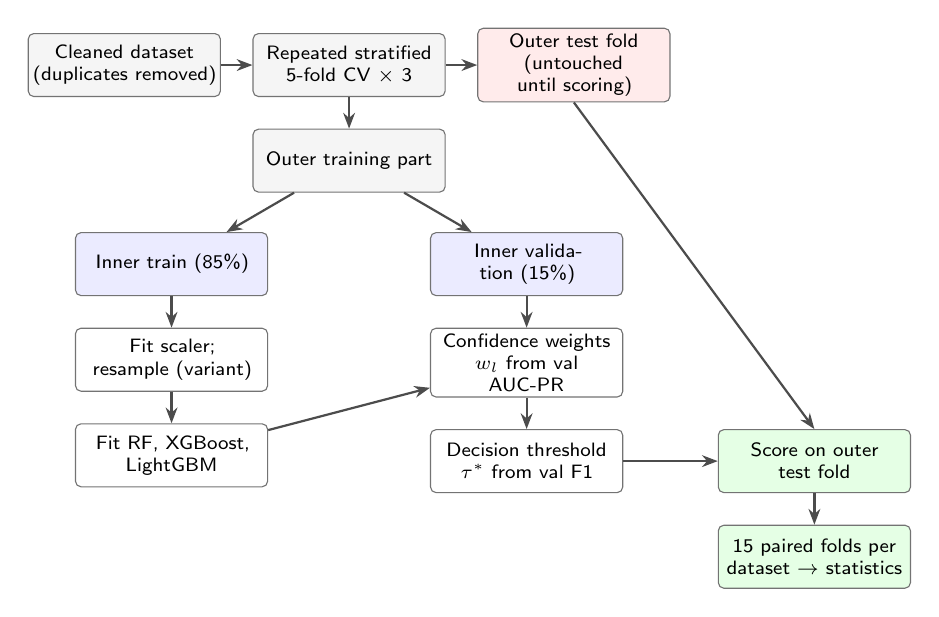
\begin{tikzpicture}[
    font=\sffamily\scriptsize,
    box/.style={draw=black!55, rounded corners=2pt, fill=#1, align=center, minimum height=8mm,
                text width=23mm, inner sep=2pt},
    box/.default=white,
    arr/.style={-{Stealth[length=2mm]}, thick, black!70},
    node distance=4mm and 4mm
  ]
  \node[box=gray!8] (data) {Cleaned dataset\\(duplicates removed)};
  \node[box=gray!8, right=of data] (cv) {Repeated stratified\\5-fold CV $\times$ 3};
  \node[box=red!8, right=of cv] (test) {Outer test fold\\(untouched until scoring)};
  \node[box=gray!8, below=of cv] (train) {Outer training part};
  \node[box=blue!8, below left=5mm and -2mm of train] (tr) {Inner train (85\%)};
  \node[box=blue!8, below right=5mm and -2mm of train] (val) {Inner validation (15\%)};
  \node[box=white, below=of tr] (scale) {Fit scaler;\\resample (variant)};
  \node[box=white, below=of scale] (fit) {Fit RF, XGBoost,\\LightGBM};
  \node[box=white, below=of val] (wt) {Confidence weights\\$w_l$ from val AUC-PR};
  \node[box=white, below=of wt] (th) {Decision threshold\\$\tau^\ast$ from val F1};
  \node[box=green!10, right=12mm of th] (score) {Score on outer\\test fold};
  \node[box=green!10, below=of score] (st) {15 paired folds per\\dataset $\to$ statistics};

  \draw[arr] (data) -- (cv); \draw[arr] (cv) -- (test); \draw[arr] (cv) -- (train);
  \draw[arr] (train) -- (tr); \draw[arr] (train) -- (val);
  \draw[arr] (tr) -- (scale); \draw[arr] (scale) -- (fit);
  \draw[arr] (val) -- (wt); \draw[arr] (wt) -- (th);
  \draw[arr] (fit) -- (wt);
  \draw[arr] (th) -- (score); \draw[arr] (test.south) -- (score.north);
  \draw[arr] (score) -- (st);
\end{tikzpicture}
}
  \caption{Leakage-free protocol: scaling, resampling, weights and threshold are fitted inside the outer training
  part of each fold.}
  \label{fig:protocol}
\end{figure}

\para{Learners and metrics}
Hyperparameters were fixed in advance and are shared by all variants:
\begin{itemize}
  \item Random Forest: 300 unpruned trees;
  \item XGBoost: 300 trees, depth 6, learning rate 0.1, row and column subsampling 0.8;
  \item LightGBM: 300 trees, learning rate 0.1;
  \item all resamplers: $k=5$ neighbours.
\end{itemize}
We report minority-class F1, AUC-PR (average precision, our primary threshold-free metric), G-mean and
MCC~\cite{saito2015precision,kubat1997addressing,chicco2020advantages}. For yeast, F1, AUC-PR and G-mean are
macro-averaged.

\para{Statistics}
\begin{itemize}
  \item \textbf{Across datasets}~\cite{demsar2006statistical}: average ranks, the Friedman and Iman--Davenport
        tests~\cite{friedman1937use,iman1980approximations}, the Nemenyi critical difference, and Wilcoxon tests of
        \ars{} against each variant~\cite{wilcoxon1945individual}, Holm-corrected~\cite{holm1979simple}.
  \item \textbf{Within datasets}: the corrected resampled $t$-test~\cite{nadeau2003inference,bouckaert2004evaluating},
        because the 15 folds are correlated.
  \item \textbf{Bayesian}: correlated $t$-tests per dataset~\cite{corani2015bayesian} and signed-rank tests across
        datasets~\cite{benavoli2014bayesian}, with a ROPE of $\pm0.01$ and a decision when one region reaches posterior
        probability 0.95~\cite{benavoli2017time}.
\end{itemize}

\para{Computation}
The $28\times9\times15=3{,}780$ folds took 16.2 compute-hours on a 16-thread CPU with an RTX~3050 GPU (used by
XGBoost), from a single committed code version.

\section{Results}\label{sec:results}

\para{Overall ranking}
Table~\ref{tab:ranks} and Figure~\ref{fig:ranks} give average ranks over the 28 datasets. The Friedman test rejects
equal performance for F1 ($p=0.0018$), AUC-PR ($p=1.4\times10^{-4}$) and MCC ($p=5.8\times10^{-4}$), but not for
G-mean ($p=0.11$). The differences come almost entirely from the two most aggressive global resamplers, SMOTE-ENN
(AUC-PR rank 7.11) and ADASYN (6.16). The other seven variants lie within about one rank of each other. \ars{} ranks
5th on AUC-PR (4.70), 4th on G-mean and 7th on F1 and MCC, while training \emph{without} resampling ranks first on
AUC-PR (4.21) and MCC (4.29).

\begin{table}
  \centering
  \caption{Average rank over 28 datasets (1 = best; best in bold) and Friedman $p$-values.}
  \label{tab:ranks}
  \footnotesize
  \setlength{\tabcolsep}{4pt}
  \begin{tabular}{lrrrr}
\toprule
Variant & F1 & AUC-PR & G-mean & MCC \\
\midrule
No resampling & 4.68 & \textbf{4.21} & 4.96 & \textbf{4.29} \\
SMOTE & 4.68 & 4.23 & 4.93 & 4.64 \\
ARS (DBSCAN) & \textbf{4.20} & 4.29 & 4.52 & 4.55 \\
SMOTE-Tomek & 4.25 & 4.30 & \textbf{4.39} & 4.36 \\
\textbf{ARS-Stack} & 4.79 & 4.70 & 4.61 & 4.82 \\
Equal-weight avg. & 4.79 & 4.71 & 4.46 & 4.64 \\
Meta-learner stacking & 4.55 & 5.29 & 5.02 & 4.45 \\
ADASYN & 6.32 & 6.16 & 6.36 & 6.25 \\
SMOTE-ENN & 6.75 & 7.11 & 5.75 & 7.00 \\
\midrule
Friedman $p$ & 0.0018 & 0.00014 & 0.11 & 0.00058 \\
\bottomrule
\end{tabular}

\end{table}

\begin{widefigure}
  \centering
  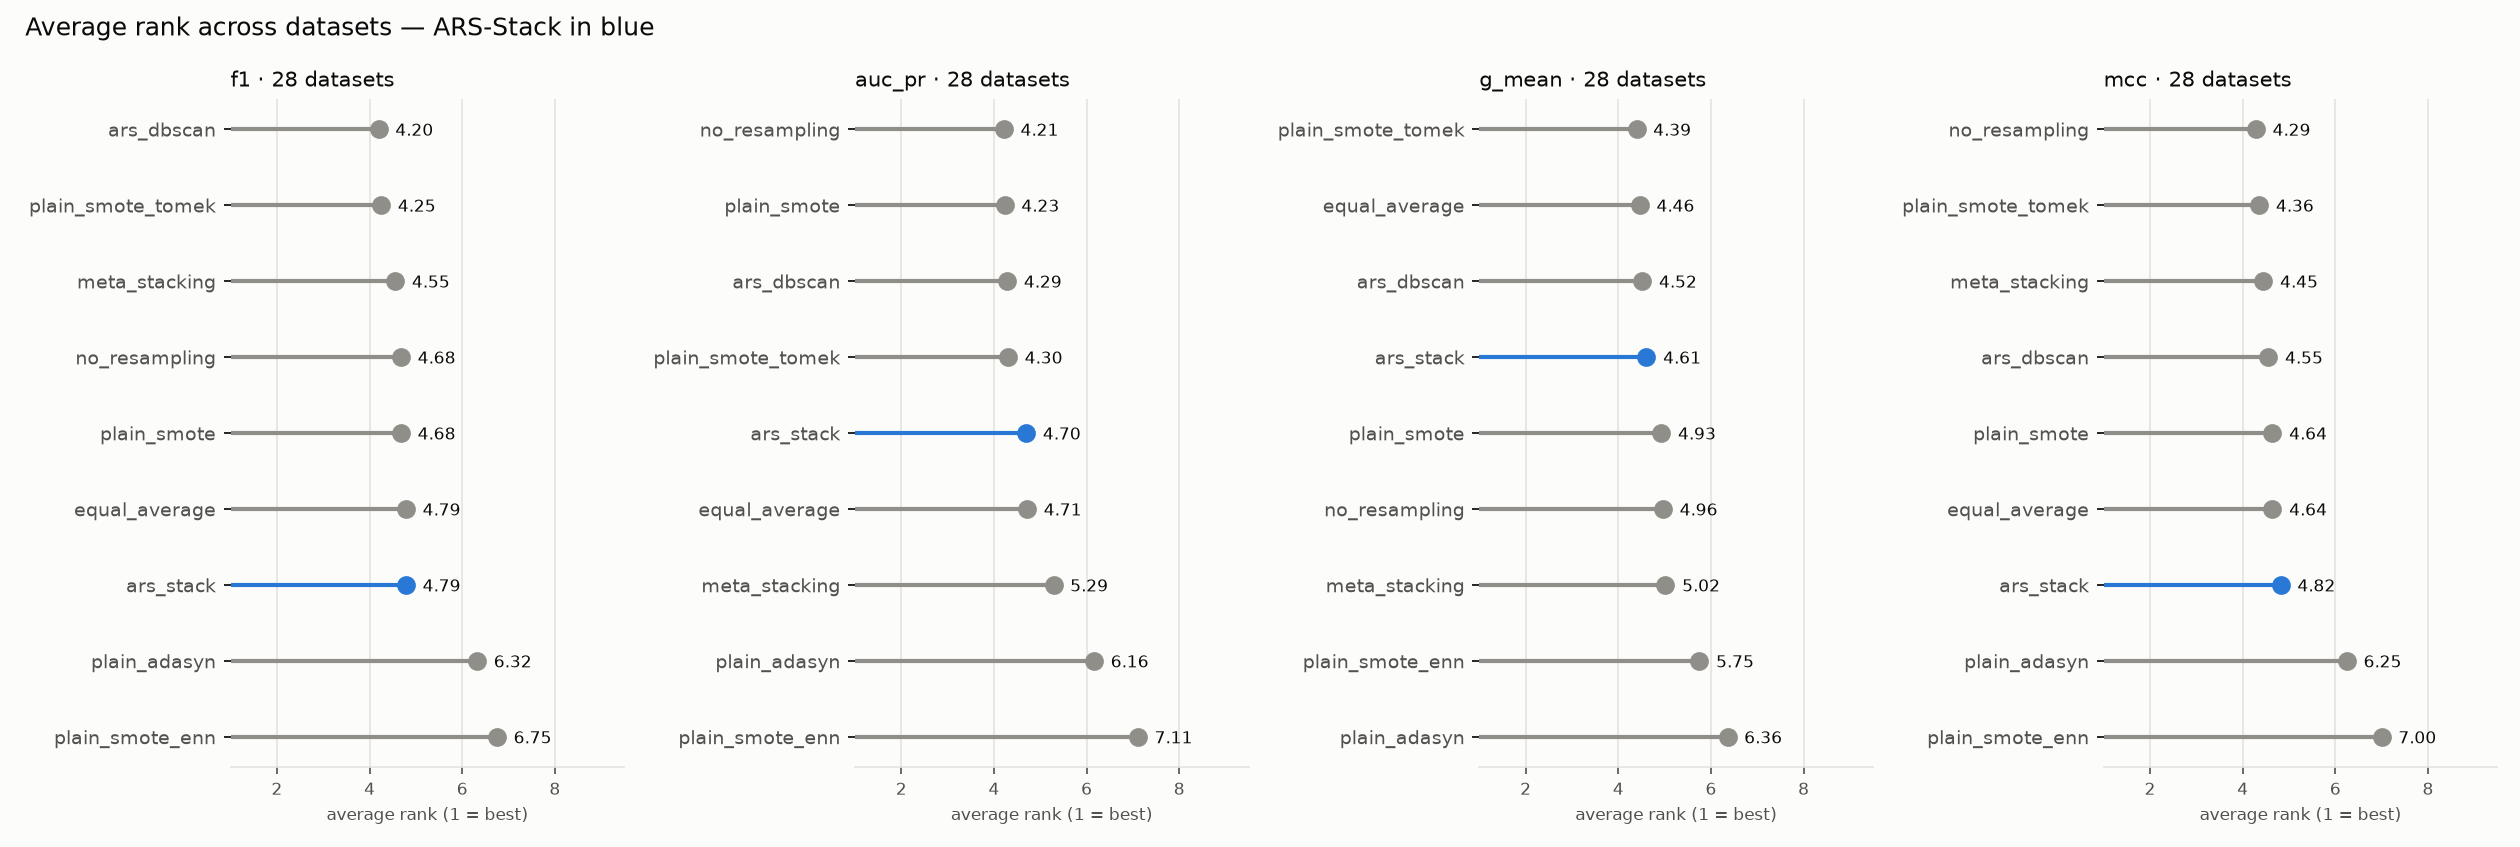
\includegraphics[width=\linewidth]{figures/average_ranks.png}
  \caption{Average rank per metric over 28 datasets (1 = best; \ars{} highlighted). Apart from SMOTE-ENN and ADASYN,
  all variants lie within about one rank of each other.}
  \label{fig:ranks}
\end{widefigure}

\para{Critical differences}
With 9 methods and 28 datasets, the Nemenyi critical difference is 2.27 ranks (Figure~\ref{fig:cd}). For AUC-PR,
SMOTE-ENN is significantly worse than every method ranked 4.84 or better, including \ars{}. For F1, it is
significantly worse only than ARS with DBSCAN (4.20) and SMOTE-Tomek (4.25), and \ars{} (4.79) is not separated from
it. No other pair of methods differs significantly.

\begin{widefigure}
  \centering
  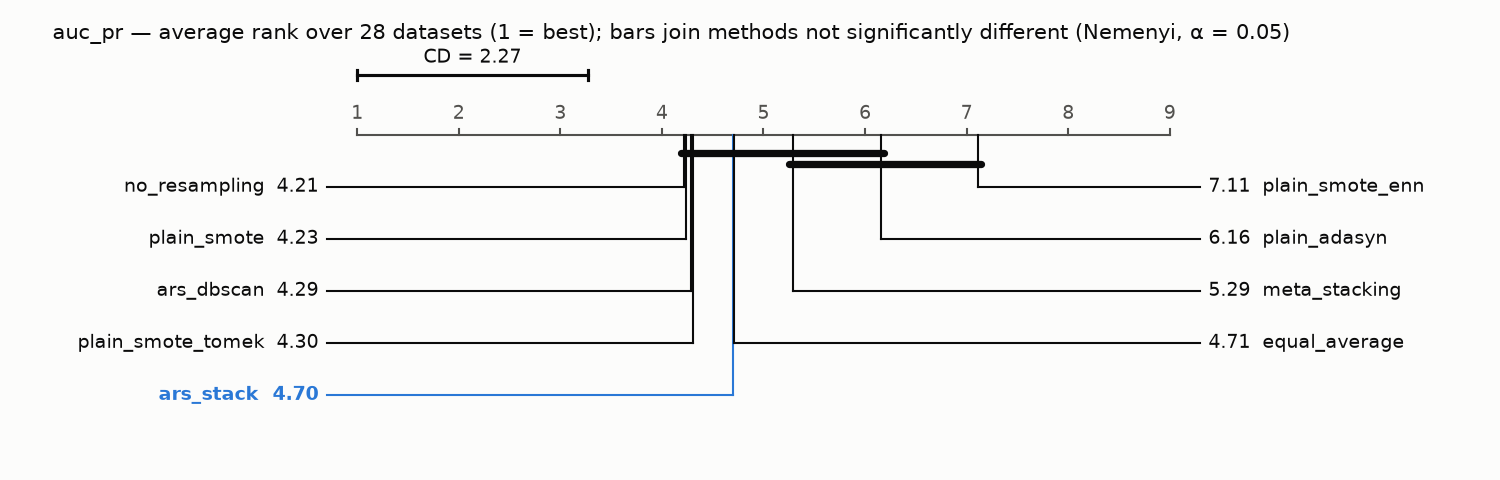
\includegraphics[width=0.49\linewidth]{figures/cd_auc_pr.png}\hfill
  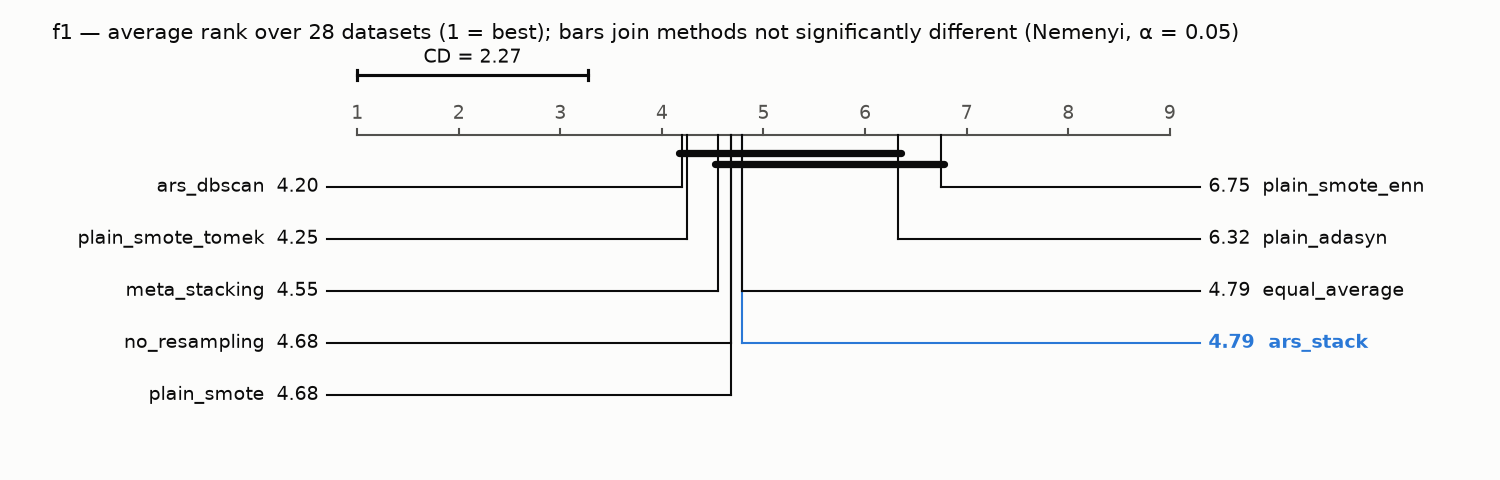
\includegraphics[width=0.49\linewidth]{figures/cd_f1.png}
  \caption{Critical-difference diagrams for AUC-PR (left) and F1 (right). Methods joined by a bar are not
  significantly different (Nemenyi, $\alpha=0.05$, CD $=2.27$).}
  \label{fig:cd}
\end{widefigure}

\para{Pairwise comparisons}
Holm-corrected Wilcoxon tests on per-dataset means (Table~\ref{tab:cross}) show \ars{} significantly better than
SMOTE-ENN on F1 (21 wins/7 losses, $p_{\mathrm{Holm}}=0.041$), AUC-PR (22/6, $p=0.049$) and MCC (22/6, $p=0.041$). Its
edge over ADASYN (19/9) does not survive correction ($p=0.089$ on F1). Against all other variants the win/loss counts
are near even, and the mean AUC-PR differences are small: $-0.0045$ against SMOTE, $-0.0062$ against No resampling,
and $+0.0001$ against equal weighting.

\begin{widetable}
  \centering
  \caption{\ars{} against each variant over 28 datasets: wins/ties/losses of \ars{}, mean difference $\Delta$
  (\ars{} $-$ baseline) and Holm-corrected Wilcoxon $p$ (bold: $p<0.05$).}
  \label{tab:cross}
  \footnotesize
  \setlength{\tabcolsep}{3.5pt}
  \begin{tabular}{lrrrrrrrrr}
\toprule
 & \multicolumn{3}{c}{F1} & \multicolumn{3}{c}{AUC-PR} & \multicolumn{3}{c}{MCC} \\
\cmidrule(lr){2-4}\cmidrule(lr){5-7}\cmidrule(lr){8-10}
ARS-Stack vs. & W/T/L & $\Delta$ & $p_{\mathrm{Holm}}$ & W/T/L & $\Delta$ & $p_{\mathrm{Holm}}$ & W/T/L & $\Delta$ & $p_{\mathrm{Holm}}$ \\
\midrule
Equal-weight avg. & 11/8/9 & +0.0003 & 1 & 12/3/13 & +0.0001 & 1 & 9/8/11 & +0.0003 & 1 \\
Meta-learner stacking & 13/3/12 & +0.0011 & 1 & 16/1/11 & +0.0019 & 0.983 & 12/3/13 & +0.0005 & 1 \\
ARS (DBSCAN) & 10/5/13 & +0.0017 & 1 & 9/5/14 & -0.0011 & 1 & 12/5/11 & +0.0024 & 1 \\
SMOTE & 11/0/17 & +0.0011 & 1 & 12/0/16 & -0.0045 & 0.879 & 11/0/17 & +0.0025 & 1 \\
SMOTE-Tomek & 11/0/17 & +0.0003 & 1 & 14/0/14 & -0.0041 & 0.983 & 11/0/17 & +0.0012 & 1 \\
ADASYN & 19/0/9 & +0.0088 & 0.089 & 19/0/9 & +0.0014 & 0.983 & 19/0/9 & +0.0079 & 0.117 \\
SMOTE-ENN & 21/0/7 & +0.0216 & \textbf{0.041} & 22/0/6 & +0.0176 & \textbf{0.048} & 22/0/6 & +0.0222 & \textbf{0.041} \\
No resampling & 14/0/14 & +0.0066 & 1 & 12/0/16 & -0.0062 & 1 & 13/0/15 & +0.0025 & 1 \\
\bottomrule
\end{tabular}

\end{widetable}

\para{Bayesian analysis}
The Bayesian signed-rank test (Table~\ref{tab:bayes}) can support equivalence. It shows:
\begin{itemize}
  \item \textbf{Practically better:} \ars{} beats SMOTE-ENN on F1 ($P=0.96$), AUC-PR ($0.98$) and MCC ($0.99$).
  \item \textbf{Practically equivalent} ($P(=)\geq0.95$) to SMOTE, SMOTE-Tomek, ARS with DBSCAN, equal-weight
        averaging and meta-learner stacking on all three metrics, and to ADASYN on AUC-PR and MCC.
  \item \textbf{Undecided} against No resampling. Equivalence is the most probable outcome ($P(=)=0.79$--$0.85$), and on
        AUC-PR No resampling is more likely better than worse (0.15 versus 0.003).
\end{itemize}
The per-dataset Bayesian correlated $t$-tests are mostly undecided with 15 folds. Where they decide, they confirm the
same picture: 76 of 112 dataset--metric pairs are equivalent to equal-weight averaging, and all 12 decided pairs against
SMOTE-ENN favour \ars{}.

\begin{widetable}
  \centering
  \caption{Bayesian signed-rank test over 28 datasets (ROPE $\pm0.01$): posterior probability that the baseline is
  practically better / equivalent / worse than \ars{}; a verdict needs $P\geq0.95$.}
  \label{tab:bayes}
  \footnotesize
  \setlength{\tabcolsep}{2.5pt}
  \begin{tabular}{lclclcl}
\toprule
 & \multicolumn{2}{c}{F1} & \multicolumn{2}{c}{AUC-PR} & \multicolumn{2}{c}{MCC} \\
\cmidrule(lr){2-3}\cmidrule(lr){4-5}\cmidrule(lr){6-7}
ARS-Stack vs. & $P(<)/P(=)/P(>)$ & Verdict & $P(<)/P(=)/P(>)$ & Verdict & $P(<)/P(=)/P(>)$ & Verdict \\
\midrule
Equal-weight avg. & 0.00/1.00/0.00 & equiv. & 0.00/1.00/0.00 & equiv. & 0.00/1.00/0.00 & equiv. \\
Meta-learner stacking & 0.00/1.00/0.00 & equiv. & 0.00/1.00/0.00 & equiv. & 0.00/1.00/0.00 & equiv. \\
ARS (DBSCAN) & 0.00/1.00/0.00 & equiv. & 0.00/1.00/0.00 & equiv. & 0.00/1.00/0.00 & equiv. \\
SMOTE & 0.00/1.00/0.00 & equiv. & 0.01/0.99/0.00 & equiv. & 0.00/0.99/0.01 & equiv. \\
SMOTE-Tomek & 0.00/1.00/0.00 & equiv. & 0.00/1.00/0.00 & equiv. & 0.00/0.99/0.00 & equiv. \\
ADASYN & 0.00/0.95/0.05 & undecided & 0.00/1.00/0.00 & equiv. & 0.00/0.98/0.02 & equiv. \\
SMOTE-ENN & 0.00/0.04/0.96 & ARS better & 0.00/0.02/0.98 & ARS better & 0.00/0.01/0.99 & ARS better \\
No resampling & 0.03/0.79/0.18 & undecided & 0.15/0.85/0.00 & undecided & 0.10/0.82/0.08 & undecided \\
\bottomrule
\end{tabular}

\end{widetable}

\para{Per-dataset results}
Table~\ref{tab:perds} lists every dataset with its characteristics and mean AUC-PR, ordered by minority-class size.
No resampling has the highest AUC-PR on 12 of the 28 datasets. On webpage, us\_crime, scene and wine\_quality, every
resampling variant loses 0.03--0.09 AUC-PR against it. Resampling wins mostly on datasets with tiny minority classes
(arrhythmia, oil, ozone\_level, abalone\_19). Saturated datasets (pen\_digits, car\_eval\_4, letter\_img,
optical\_digits) leave all variants within 0.002 of each other, except SMOTE-ENN on car\_eval\_4.

For the core datasets (Table~\ref{tab:core}), the variants on creditcard differ by less than a standard deviation, and
No resampling is best on mammography for every metric except G-mean. On 10-class yeast, resampling gives the largest
gains in the study: macro-F1 rises from 0.441 to 0.524 and G-mean from 0.642 to 0.708. SMOTE-ENN, by contrast,
collapses MCC to 0.388.

\begin{widetable}
  \centering
  \caption{Datasets and mean AUC-PR over 15 folds (best per dataset in bold), ordered by minority-class size. $n$:
  samples after duplicate removal; $d$: features; Min.: minority (smallest-class) size; IR: imbalance ratio.
  Core datasets are marked $^\ast$.}
  \label{tab:perds}
  \scriptsize
  \setlength{\tabcolsep}{3pt}
  \begin{tabular}{lrrrrrrrrrrr}
\toprule
 & & & & & \multicolumn{7}{c}{Mean AUC-PR} \\
\cmidrule(l){6-12}
Dataset & $n$ & $d$ & Min. & IR & None & SMOTE & SM-Tomek & ADASYN & SM-ENN & Meta & ARS \\
\midrule
yeast (10-class)$^\ast$ & 1,453 & 8 & 5 & 87.6 & 0.591 & \textbf{0.599} & 0.599 & 0.586 & 0.566 & 0.579 & 0.597 \\
libras\_move & 330 & 90 & 24 & 12.8 & 0.881 & 0.895 & 0.895 & 0.881 & 0.878 & \textbf{0.899} & 0.894 \\
arrhythmia & 452 & 278 & 25 & 17.1 & 0.815 & 0.833 & 0.833 & 0.837 & 0.783 & 0.840 & \textbf{0.843} \\
abalone\_19 & 4,177 & 10 & 32 & 129.5 & 0.049 & 0.068 & \textbf{0.075} & 0.056 & 0.056 & 0.058 & 0.055 \\
ecoli & 336 & 7 & 35 & 8.6 & 0.702 & 0.714 & 0.682 & \textbf{0.719} & 0.651 & 0.686 & 0.682 \\
oil & 937 & 49 & 41 & 21.9 & 0.580 & \textbf{0.622} & \textbf{0.622} & 0.620 & 0.573 & 0.603 & 0.600 \\
spectrometer & 531 & 93 & 45 & 10.8 & \textbf{0.913} & 0.878 & 0.885 & 0.854 & 0.858 & 0.865 & 0.865 \\
solar\_flare\_m0 & 412 & 32 & 58 & 6.1 & 0.186 & 0.177 & 0.178 & 0.175 & \textbf{0.246} & 0.192 & 0.193 \\
car\_eval\_4 & 1,728 & 21 & 65 & 25.6 & 0.999 & 1.000 & 1.000 & 1.000 & 0.972 & \textbf{1.000} & \textbf{1.000} \\
ozone\_level & 2,536 & 72 & 73 & 33.7 & 0.321 & 0.369 & 0.369 & 0.361 & \textbf{0.385} & 0.355 & 0.356 \\
car\_eval\_34 & 1,728 & 21 & 134 & 11.9 & 0.990 & 0.989 & 0.989 & 0.990 & 0.973 & \textbf{0.990} & 0.990 \\
us\_crime & 1,994 & 100 & 150 & 12.3 & \textbf{0.594} & 0.546 & 0.548 & 0.546 & 0.523 & 0.549 & 0.550 \\
scene & 2,400 & 294 & 173 & 12.9 & \textbf{0.271} & 0.242 & 0.245 & 0.239 & 0.210 & 0.223 & 0.226 \\
wine\_quality & 3,961 & 11 & 173 & 21.9 & \textbf{0.322} & 0.282 & 0.280 & 0.274 & 0.271 & 0.251 & 0.249 \\
yeast\_ml8 & 2,417 & 103 & 178 & 12.6 & \textbf{0.108} & 0.104 & 0.104 & 0.103 & 0.105 & 0.108 & 0.107 \\
thyroid\_sick & 3,771 & 52 & 231 & 15.3 & \textbf{0.954} & 0.946 & 0.947 & 0.947 & 0.893 & 0.944 & 0.946 \\
mammography$^\ast$ & 7,849 & 6 & 254 & 29.9 & \textbf{0.780} & 0.766 & 0.767 & 0.739 & 0.722 & 0.760 & 0.763 \\
sick\_euthyroid & 3,109 & 42 & 285 & 9.9 & \textbf{0.898} & 0.897 & 0.897 & 0.896 & 0.868 & 0.897 & 0.896 \\
abalone & 4,177 & 10 & 391 & 9.7 & 0.297 & 0.302 & 0.305 & 0.298 & \textbf{0.317} & 0.291 & 0.290 \\
creditcard$^\ast$ & 283,726 & 30 & 473 & 598.8 & 0.840 & \textbf{0.844} & \textbf{0.844} & 0.836 & 0.830 & 0.843 & 0.843 \\
optical\_digits & 5,620 & 64 & 554 & 9.1 & \textbf{0.995} & 0.995 & 0.995 & 0.994 & 0.994 & 0.995 & 0.995 \\
coil\_2000 & 8,380 & 85 & 568 & 13.8 & 0.126 & 0.125 & 0.124 & 0.124 & \textbf{0.140} & 0.119 & 0.124 \\
isolet & 7,797 & 617 & 600 & 12.0 & \textbf{0.967} & 0.962 & 0.962 & 0.960 & 0.867 & 0.959 & 0.962 \\
satimage & 6,435 & 36 & 626 & 9.3 & 0.809 & \textbf{0.811} & 0.811 & 0.805 & 0.728 & 0.806 & 0.811 \\
letter\_img & 18,668 & 16 & 640 & 28.2 & \textbf{0.996} & 0.995 & 0.995 & 0.995 & 0.995 & 0.995 & 0.995 \\
webpage & 34,780 & 300 & 981 & 34.5 & \textbf{0.855} & 0.814 & 0.814 & 0.788 & 0.761 & 0.788 & 0.814 \\
pen\_digits & 10,992 & 16 & 1,055 & 9.4 & 0.998 & 0.998 & 0.998 & 0.997 & 0.998 & \textbf{0.999} & \textbf{0.999} \\
protein\_homo & 144,968 & 74 & 1,251 & 114.9 & 0.885 & 0.901 & 0.901 & 0.888 & 0.893 & 0.901 & \textbf{0.902} \\
\midrule
Mean & & & & & 0.669 & 0.667 & 0.667 & 0.661 & 0.645 & 0.660 & 0.662 \\
\bottomrule
\end{tabular}

\end{widetable}

\begin{table}
  \centering
  \caption{Core datasets: mean $\pm$ standard deviation over 15 folds (best in bold).}
  \label{tab:core}
  \scriptsize
  \setlength{\tabcolsep}{2pt}
  \resizebox{\linewidth}{!}{\begin{tabular}{lrrrr}
\toprule
Variant & F1 & AUC-PR & G-mean & MCC \\
\midrule
\multicolumn{5}{l}{\textit{creditcard}} \\
\quad No resampling & \textbf{0.852 $\pm$ 0.023} & 0.840 $\pm$ 0.027 & 0.889 $\pm$ 0.019 & \textbf{0.855 $\pm$ 0.023} \\
\quad SMOTE & 0.846 $\pm$ 0.026 & 0.844 $\pm$ 0.028 & \textbf{0.890 $\pm$ 0.018} & 0.848 $\pm$ 0.026 \\
\quad SMOTE-ENN & 0.829 $\pm$ 0.031 & 0.830 $\pm$ 0.032 & 0.888 $\pm$ 0.024 & 0.830 $\pm$ 0.031 \\
\quad Meta-learner stacking & 0.846 $\pm$ 0.022 & 0.843 $\pm$ 0.026 & 0.885 $\pm$ 0.016 & 0.849 $\pm$ 0.022 \\
\quad ARS-Stack & 0.846 $\pm$ 0.022 & 0.843 $\pm$ 0.027 & 0.886 $\pm$ 0.015 & 0.848 $\pm$ 0.022 \\
\multicolumn{5}{l}{\textit{mammography}} \\
\quad No resampling & \textbf{0.709 $\pm$ 0.049} & \textbf{0.780 $\pm$ 0.042} & 0.824 $\pm$ 0.044 & \textbf{0.703 $\pm$ 0.050} \\
\quad SMOTE & 0.699 $\pm$ 0.041 & 0.766 $\pm$ 0.047 & 0.815 $\pm$ 0.038 & 0.693 $\pm$ 0.041 \\
\quad SMOTE-ENN & 0.662 $\pm$ 0.040 & 0.722 $\pm$ 0.058 & \textbf{0.833 $\pm$ 0.043} & 0.654 $\pm$ 0.040 \\
\quad Meta-learner stacking & 0.699 $\pm$ 0.051 & 0.760 $\pm$ 0.046 & 0.813 $\pm$ 0.050 & 0.696 $\pm$ 0.049 \\
\quad ARS-Stack & 0.694 $\pm$ 0.052 & 0.763 $\pm$ 0.046 & 0.801 $\pm$ 0.048 & 0.693 $\pm$ 0.049 \\
\multicolumn{5}{l}{\textit{yeast (10-class)}} \\
\quad No resampling & 0.441 $\pm$ 0.043 & 0.591 $\pm$ 0.057 & 0.642 $\pm$ 0.029 & 0.444 $\pm$ 0.041 \\
\quad SMOTE & 0.520 $\pm$ 0.060 & 0.599 $\pm$ 0.038 & 0.701 $\pm$ 0.043 & 0.447 $\pm$ 0.034 \\
\quad SMOTE-ENN & 0.461 $\pm$ 0.045 & 0.566 $\pm$ 0.047 & \textbf{0.725 $\pm$ 0.043} & 0.388 $\pm$ 0.032 \\
\quad Meta-learner stacking & 0.527 $\pm$ 0.062 & 0.579 $\pm$ 0.062 & 0.710 $\pm$ 0.041 & \textbf{0.471 $\pm$ 0.025} \\
\quad ARS-Stack & 0.524 $\pm$ 0.064 & 0.597 $\pm$ 0.041 & 0.708 $\pm$ 0.045 & 0.447 $\pm$ 0.032 \\
\bottomrule
\end{tabular}
}
\end{table}

\iffullversion
\begin{figure}
  \centering
  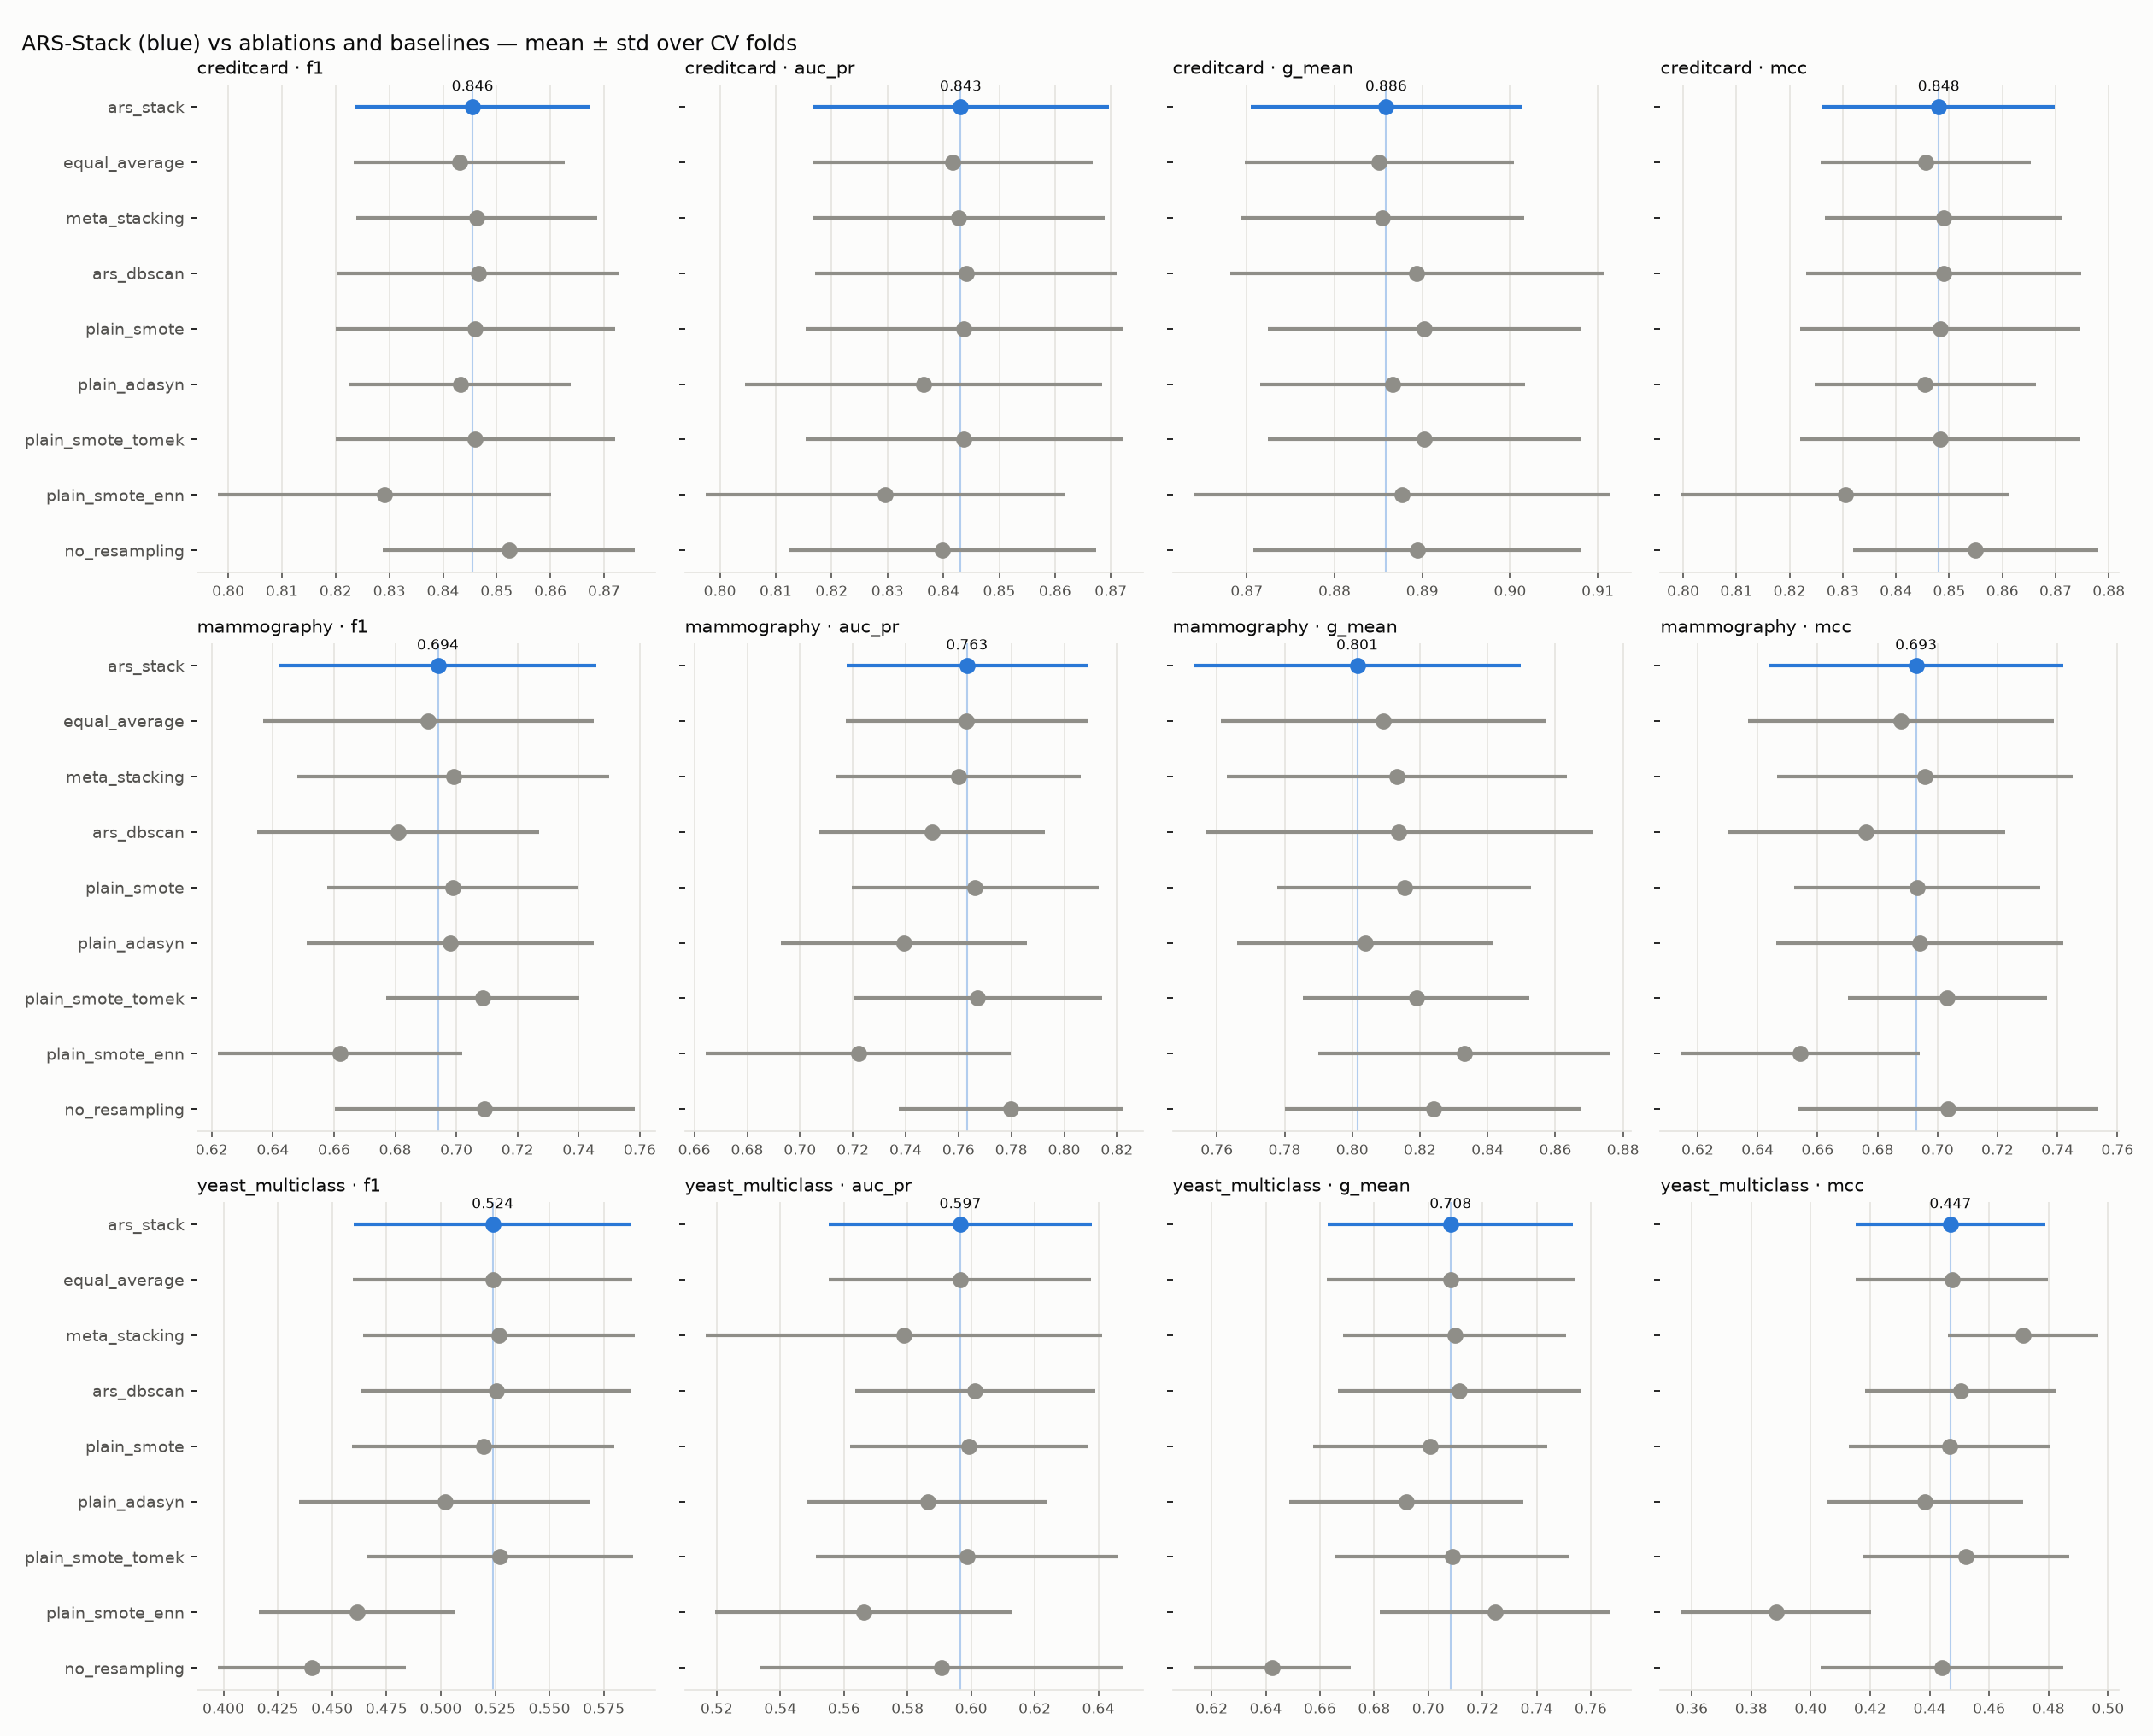
\includegraphics[width=0.78\linewidth]{figures/core_comparison.png}
  \caption{Core datasets: mean $\pm$ standard deviation over 15 folds for all nine variants and four metrics
  (\ars{} highlighted). Fold-to-fold spread exceeds most differences between variants.}
  \label{fig:core}
\end{figure}
\fi

\para{Literature baselines}
Reproducing the ``SMOTE + learner'' baselines of our review on a fixed split with a 0.5 threshold
(Table~\ref{tab:lit}) gives lower scores than published: creditcard F1 is 0.78--0.83 against the reported
0.89--0.915. Three leakage-free choices account for the gap: we remove duplicates, apply SMOTE only after splitting,
and hold the test set out. Oversampling before the split, common in applied work, lets synthetic interpolations of
test points leak into training. The comparison is indicative only, since the published splits differ.

\begin{table}
  \centering
  \caption{Literature baselines on a fixed split (0.5 threshold) versus reported values.}
  \label{tab:lit}
  \scriptsize
  \setlength{\tabcolsep}{2pt}
  \resizebox{\linewidth}{!}{\begin{tabular}{lllrrr}
\toprule
Dataset & Model & Source & F1 & AUC-PR & MCC \\
\midrule
creditcard & RandomForest + SMOTE & ours & 0.832 & 0.821 & 0.836 \\
creditcard & XGBoost + SMOTE & ours & 0.775 & 0.818 & 0.775 \\
creditcard & Simple Stacking (RF+XGB, LR meta) + SMOTE & ours & 0.815 & 0.823 & 0.815 \\
creditcard & Paper 7: xgboost & reported & 0.890 & 0.930 & -- \\
creditcard & Paper 7: easyensemble & reported & 0.870 & -- & -- \\
creditcard & Paper 9: stacking & reported & -- & -- & -- \\
creditcard & Paper 10: stacking smote tomek & reported & 0.915 & 0.900 & -- \\
mammography & RandomForest + SMOTE & ours & 0.615 & 0.606 & 0.602 \\
mammography & XGBoost + SMOTE & ours & 0.630 & 0.639 & 0.618 \\
mammography & Simple Stacking (RF+XGB, LR meta) + SMOTE & ours & 0.647 & 0.636 & 0.635 \\
\bottomrule
\end{tabular}
}
\end{table}

\section{Why Does Adaptive Selection Not Help?}\label{sec:analysis}

\para{What the selector chose}
Over the 420 \ars{} folds, the minority classes produced 970 clusters. The resampler applied was SMOTE-Tomek for 33\%
of them, SMOTE for 30\%, SMOTE-ENN for 29\%, ADASYN for 6\% and random oversampling for 2\%.
Figure~\ref{fig:usage} shows that the choice is effectively made per \emph{dataset}. On 11 datasets, one resampler is
used for every cluster in every fold. The clustering does split the minority class, into 1.8 clusters on average and
into several clusters in 57\% of folds, but clusters of the same dataset receive similar scores and hence the same
rule. DBSCAN always returned a single cluster, yet ARS with DBSCAN matches the $k$-means version (F1 rank 4.20 versus
4.79). Per-cluster heterogeneity is not what drives performance.

\begin{figure}
  \centering
  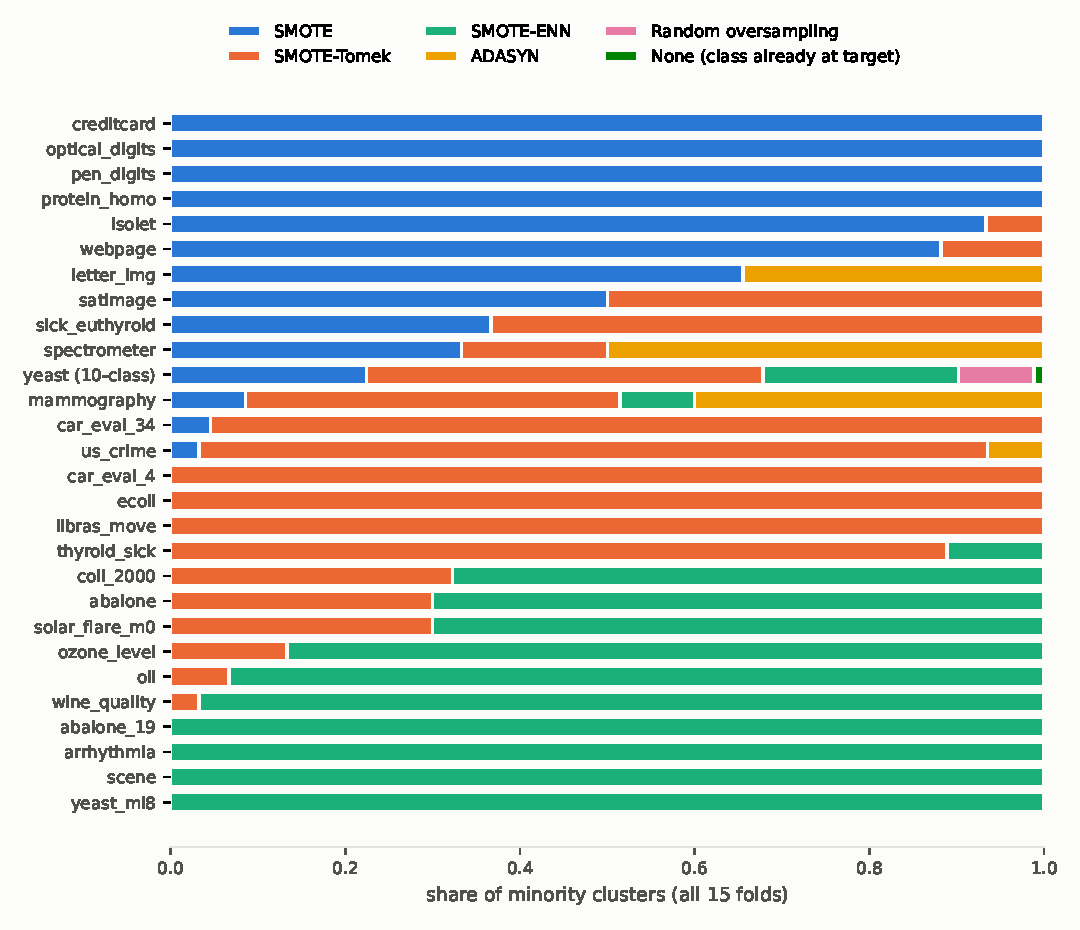
\includegraphics[width=\usagefigwidth]{figures/resampler_usage.pdf}
  \caption{Resampler applied by \ars{} per minority cluster, as a share over the 15 folds of each dataset. Most
  datasets are dominated by one resampler.}
  \label{fig:usage}
\end{figure}

\para{SMOTE-Tomek is SMOTE}
After 1:1 SMOTE, synthetic points fill the minority region so densely that almost no cross-class nearest-neighbour
pairs (Tomek links) remain. Global SMOTE-Tomek gave \emph{bit-identical} results to SMOTE on 280 of 420 folds, and on
all folds of 12 datasets, while its cleaning step cost up to 114\,s per creditcard fold. \ars{}'s most frequent choice
is therefore effectively SMOTE, and its real candidate pool is dominated by SMOTE.

\para{Confidence weighting is equal weighting}
The three learners reach similar validation AUC-PR, so the weights of Eq.~\ref{eq:weights} stay near $1/3$. The
median gap between the largest and smallest weight is 0.022 (90th percentile 0.10). \ars{} and equal-weight averaging
give identical metrics on 159 of 420 folds (mean AUC-PR difference $+0.0001$). The weights have nothing to correct
when the learners are this strong and this similar. Meta-learner stacking is also equivalent, at 4.6$\times$ the
compute (5.7 versus 1.2 hours).

\paragraph{When does resampling help at all?}
Figure~\ref{fig:benefit} plots, per dataset, the gain from resampling over the same ensemble without resampling,
against the minority-class size:
\begin{itemize}
  \item \textbf{$\leq75$ minority samples (10 datasets):} SMOTE improves AUC-PR on 8 (mean $+0.012$); \ars{} on 8
        (mean $+0.005$).
  \item \textbf{$>75$ minority samples (18 datasets):} SMOTE improves AUC-PR on only 5 (mean $-0.009$); \ars{} on 4
        (mean $-0.012$).
\end{itemize}
F1 and MCC show the same pattern. The Spearman correlations between gain and minority size are negative throughout
(e.g.\ $\rho=-0.48$, $p=0.010$ for \ars{} on F1), but none survives Holm correction over the 24 tests we ran. The
imbalance ratio itself is not predictive. The absolute number of minority examples, not their proportion, appears to
limit a strong learner. We report this as a consistent trend, not a confirmed effect.

\begin{widefigure}
  \centering
  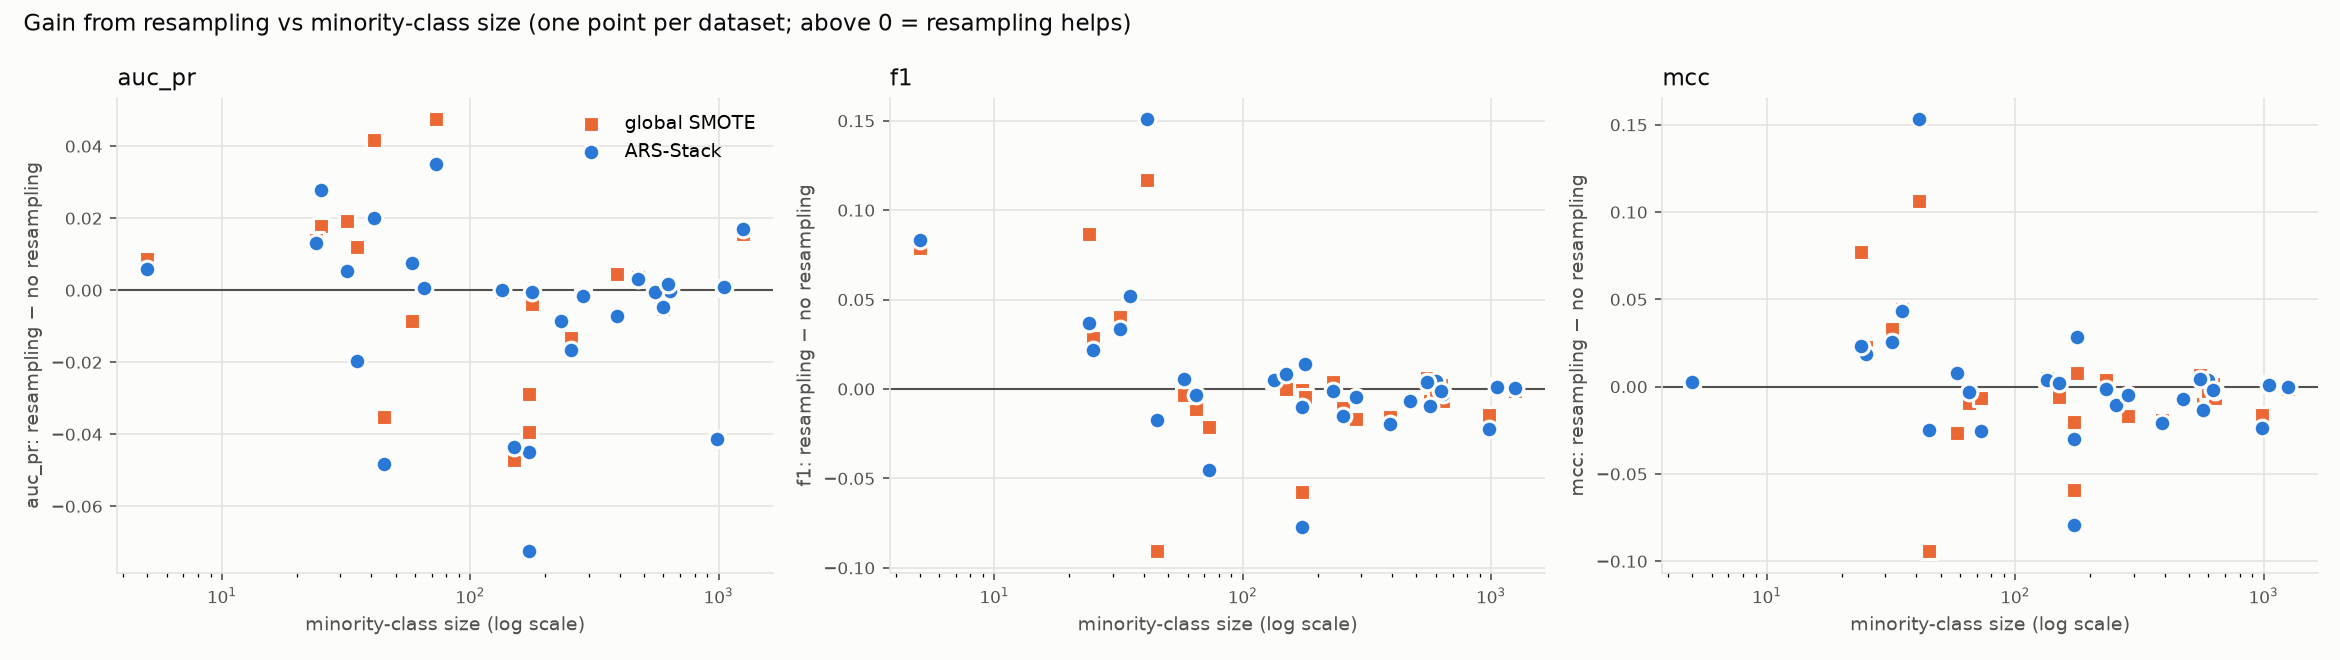
\includegraphics[width=\linewidth]{figures/resampling_benefit.png}
  \caption{Gain from resampling (global SMOTE, \ars{}) over no resampling versus minority-class size (log scale), one
  point per dataset. Resampling tends to help below about 75 minority samples and to be neutral or harmful above.}
  \label{fig:benefit}
\end{widefigure}

\para{Pilot: validated selection}
Perhaps hand-written rules are just a poor selector. To test this, we replaced them with \emph{validated selection}:
the method (no resampling, global SMOTE, or \ars{}'s adaptive resampling) and the amount
($\beta\in\{0.1,0.25,0.5,1\}$) are chosen jointly by 3-fold inner cross-validation on the training data (LightGBM
AUC-PR), and a single cluster is kept unless the silhouette score exceeds 0.25. A control, SMOTE-Select, runs the same
search without the adaptive option.

To avoid tuning on the reported benchmark, the datasets were split into 14 development and 14 held-out sets,
stratified by minority size and imbalance. The pilot used 12 development datasets and 5 folds, all on one machine.
That matters: repeating an identical configuration on different hardware moved AUC-PR by 0.007 on average, as much as
the effects studied.

Table~\ref{tab:pilot} shows that validated selection repairs \ars{}'s deficit ($+0.0095$ AUC-PR over the rule-based
version) but only reaches the baselines: $+0.0006$ over No resampling (5 wins, 7 losses) and identical to SMOTE-Select.
The adaptive option adds nothing, and the chosen configurations were spread over all candidates, a sign that they
perform alike. The headroom is small in any case: an oracle picking the best of No resampling, SMOTE, SMOTE-Tomek and
\ars{} per dataset in hindsight gains only $+0.008$ mean AUC-PR over No resampling. We therefore did not spend a
second full run on this design.

\begin{table}
  \centering
  \caption{Validated-selection pilot on 12 development datasets (5 folds, one machine): mean score (average rank among
  the five variants).}
  \label{tab:pilot}
  \scriptsize
  \setlength{\tabcolsep}{2pt}
  \resizebox{\linewidth}{!}{\begin{tabular}{lrrrr}
\toprule
Variant & F1 & AUC-PR & G-mean & MCC \\
\midrule
No resampling & 0.4919 (2.92) & 0.5301 (2.67) & 0.6944 (2.92) & 0.4696 (2.92) \\
SMOTE & 0.4854 (3.67) & 0.5290 (3.08) & 0.6810 (3.75) & 0.4602 (3.75) \\
ARS-Stack & 0.4920 (2.92) & 0.5212 (3.50) & 0.6937 (3.08) & 0.4651 (3.08) \\
SMOTE-Select (validated) & 0.4951 (2.71) & 0.5307 (2.83) & 0.6989 (2.46) & 0.4705 (2.62) \\
ARS-Select (validated) & 0.4921 (2.79) & 0.5307 (2.92) & 0.6907 (2.79) & 0.4669 (2.62) \\
\bottomrule
\end{tabular}
}
\end{table}

\section{Discussion}\label{sec:discussion}

\para{Implications}
For strong tree ensembles with a tuned threshold, \emph{which} oversampler is applied, and \emph{where}, matters
little (gaps G1--G2). The exception is aggressive cleaning: SMOTE-ENN, and to a lesser degree ADASYN, reliably hurt.
Two mechanisms explain this. First, a strong learner combined with a tuned threshold already makes the
precision--recall trade-off that resampling targets~\cite{elor2022smote,vandengoorbergh2022harm}. Second, once
budgets are matched and leakage removed, most resamplers produce near-identical training sets. Gap G3 fares better:
multiclass problems and datasets with a few dozen minority examples show the largest gains, and resampling research
should focus there.

\para{Five evaluation pitfalls}
Our first pipeline contained five errors, each of which would have produced a spurious improvement:
\begin{enumerate}
  \item \textbf{Unequal budgets.} Local balancing added far less synthetic data than global SMOTE (a 1:200 versus
        1:1 final ratio on creditcard), confounding resampler choice with resampling amount.
  \item \textbf{Scale-cancelled weights.} Confidence weights fed into a meta-learner are a no-op.
  \item \textbf{Rank-forced rules.} Percentile rules with one or two clusters decide by rank.
  \item \textbf{Fixed 0.5 thresholds.} These make F1, G-mean and MCC mirror the oversampling ratio.
  \item \textbf{Duplicates and pre-split resampling.} Both place near-copies of test points in the training data.
\end{enumerate}
Controlling for all five is, in our view, a minimum standard for resampling papers.

\para{Threats to validity}
\begin{itemize}
  \item \textbf{Fixed hyperparameters.} Hyperparameters and rule thresholds were fixed a priori, not tuned per
        dataset. Tuning would affect all variants alike.
  \item \textbf{Hardware non-determinism.} It exists (GPU versus CPU XGBoost), so the study ran on one machine from
        one code version.
  \item \textbf{Small validation splits.} The 15\% split is small for tiny minority classes.
  \item \textbf{External validity.} The benchmarks form a single collection. Deduplication limits comparability with
        prior work.
  \item \textbf{Learner scope.} The conclusions concern strong tree ensembles; weaker learners may benefit more from
        resampling~\cite{vanhulse2007experimental}.
  \item \textbf{Statistical power.} Per-dataset power is limited by 15 correlated folds, and the minority-size trend
        does not survive multiplicity correction.
\end{itemize}

\section{Future Work}\label{sec:future}
\begin{itemize}
  \item \textbf{Other learners.} Repeat the study with logistic regression, $k$-NN, SVMs and deep tabular models, to
        map the learner--resampler interaction.
  \item \textbf{The small-sample regime.} Test the minority-size trend in a pre-registered study on datasets with
        fewer than 100 minority examples, including multiclass ones, and add generative oversamplers.
  \item \textbf{Meta-learned selection.} Replace rules and noisy inner validation with a meta-model that predicts the
        benefit of resampling from dataset characteristics.
  \item \textbf{Combination.} Replace global confidence weights with dynamic ensemble selection~\cite{cruz2018dynamic}.
  \item \textbf{Alternatives to resampling.} Compare resampling with cost-sensitive learning, and evaluate
        calibration~\cite{vandengoorbergh2022harm}.
  \item \textbf{Analysis and deployment.} Use hierarchical Bayesian models across datasets~\cite{benavoli2017time},
        and add drift monitoring and energy accounting~\cite{plan_p10_stacking} to the served models.
\end{itemize}

\section{Conclusion}\label{sec:conclusion}
We proposed \ars{}, which selects a resampler per minority cluster from overlap and density scores and combines three
tree ensembles with confidence weights, and we evaluated it in a budget-matched, leakage-free study on 28 datasets.

\ars{} reliably beats aggressive cleaning (SMOTE-ENN). It is practically equivalent to plain SMOTE and to its own
ablations, and it cannot be separated from training without resampling. Each null result has a concrete cause:
near-uniform weights, cleaning that removes nothing after balancing, and selection that rarely varies within a
dataset. A validated-selection pilot confirms that the headroom is small, and resampling mainly pays off when minority
examples are scarce.

We hope the method, the pipeline and the five pitfalls help future work target the settings where resampling matters,
and measure its benefit fairly.

\para{Availability}
Code, configuration, per-fold results and analysis scripts are in the project repository. All datasets are public:
Kaggle~\cite{dalpozzolo2015calibrating}, imbalanced-learn~\cite{lemaitre2017imbalanced} and UCI.


\bibliographystyle{unsrtnat}
\setlength{\bibsep}{1.5pt plus 0.3ex}
\begingroup\footnotesize
\bibliography{references}
\endgroup

\end{document}
